[127~v\textsuperscript{o}] et par consequent (:~puisque son corps demeure le m\^{e}me~:) un m\^{e}me degrez de vistesse. Ainsi, supposant la surface \textit{AB}, ou le lieu o\`{u} le mobile passe, parsem\'{e} \'{e}galement de distance en distance de semblables pointes d'egale force, le lieu retardera partout \'{e}galement le mobile, et diminuera tousjours son mouuement, d'un m\^{e}me degrez de vitesse: et par consequent les \edtext{Theoremes}{\lemma{Theoremes}\Cfootnote{Vgl. N. 36.}} que j'ay baillez auront lieu.
\pend
\pstart
Il est vray pourtant que la resistence respective est compliqu\'{e}e dans le frottement avec la resistence absolue: Car imaginons la surface \textit{AB} comme perc\'{e}e en sorte que la pointe \textit{P} ne puisse seulement luy devenir parallele estant pli\'{e}e en \textit{p} mais qu'elle puisse m\^{e}me aller au dessous de la surface, jusqu'\`{a} $\pi$.
\pend
\pstart
Cela pos\'{e}, il est asseur\'{e}, qu'elle sera pouss\'{e}e d'autant plus loing, que le mouuement du mobile sera plus viste: et qu'ainsi \`{a} l'\'{e}gard de ce pli superflu du ressort qui fait la pointe \textit{P}, le mobile perdra d'autant plus de force, qu'il va avec plus de vistesse: par ce qu'il communique plus de force au ressort qu'il plie d'avantage. Et cela est vray quoyque la surface \textit{AB} ne soit point perc\'{e}e, et quoyque ce pli superflu jusqu'en $\pi$ ne puisse arriver effectivement. Car toute la masse du corps, dont \textit{AB} est la surface receuuera le choc, et empechera la pointe d'aller plus avant qu'en \textit{p}. Cependant le mobile \textit{M} ne laissera pas d'avoir perdu autant de force que si la pointe \textit{P}, avoit p\^{u} aller effectivement jusqu'en $\pi$. Puisqu'il luy a donn\'{e} une fois un choc suffisant pour le faire, sans l'obstacle qui en a \setline{26}empech\'{e} l'effect.
\pend
\vspace{1.5em}
\pstart
\noindent
\centering
    %\begin{wrapfigure}{l}{0.4\textwidth}                    
    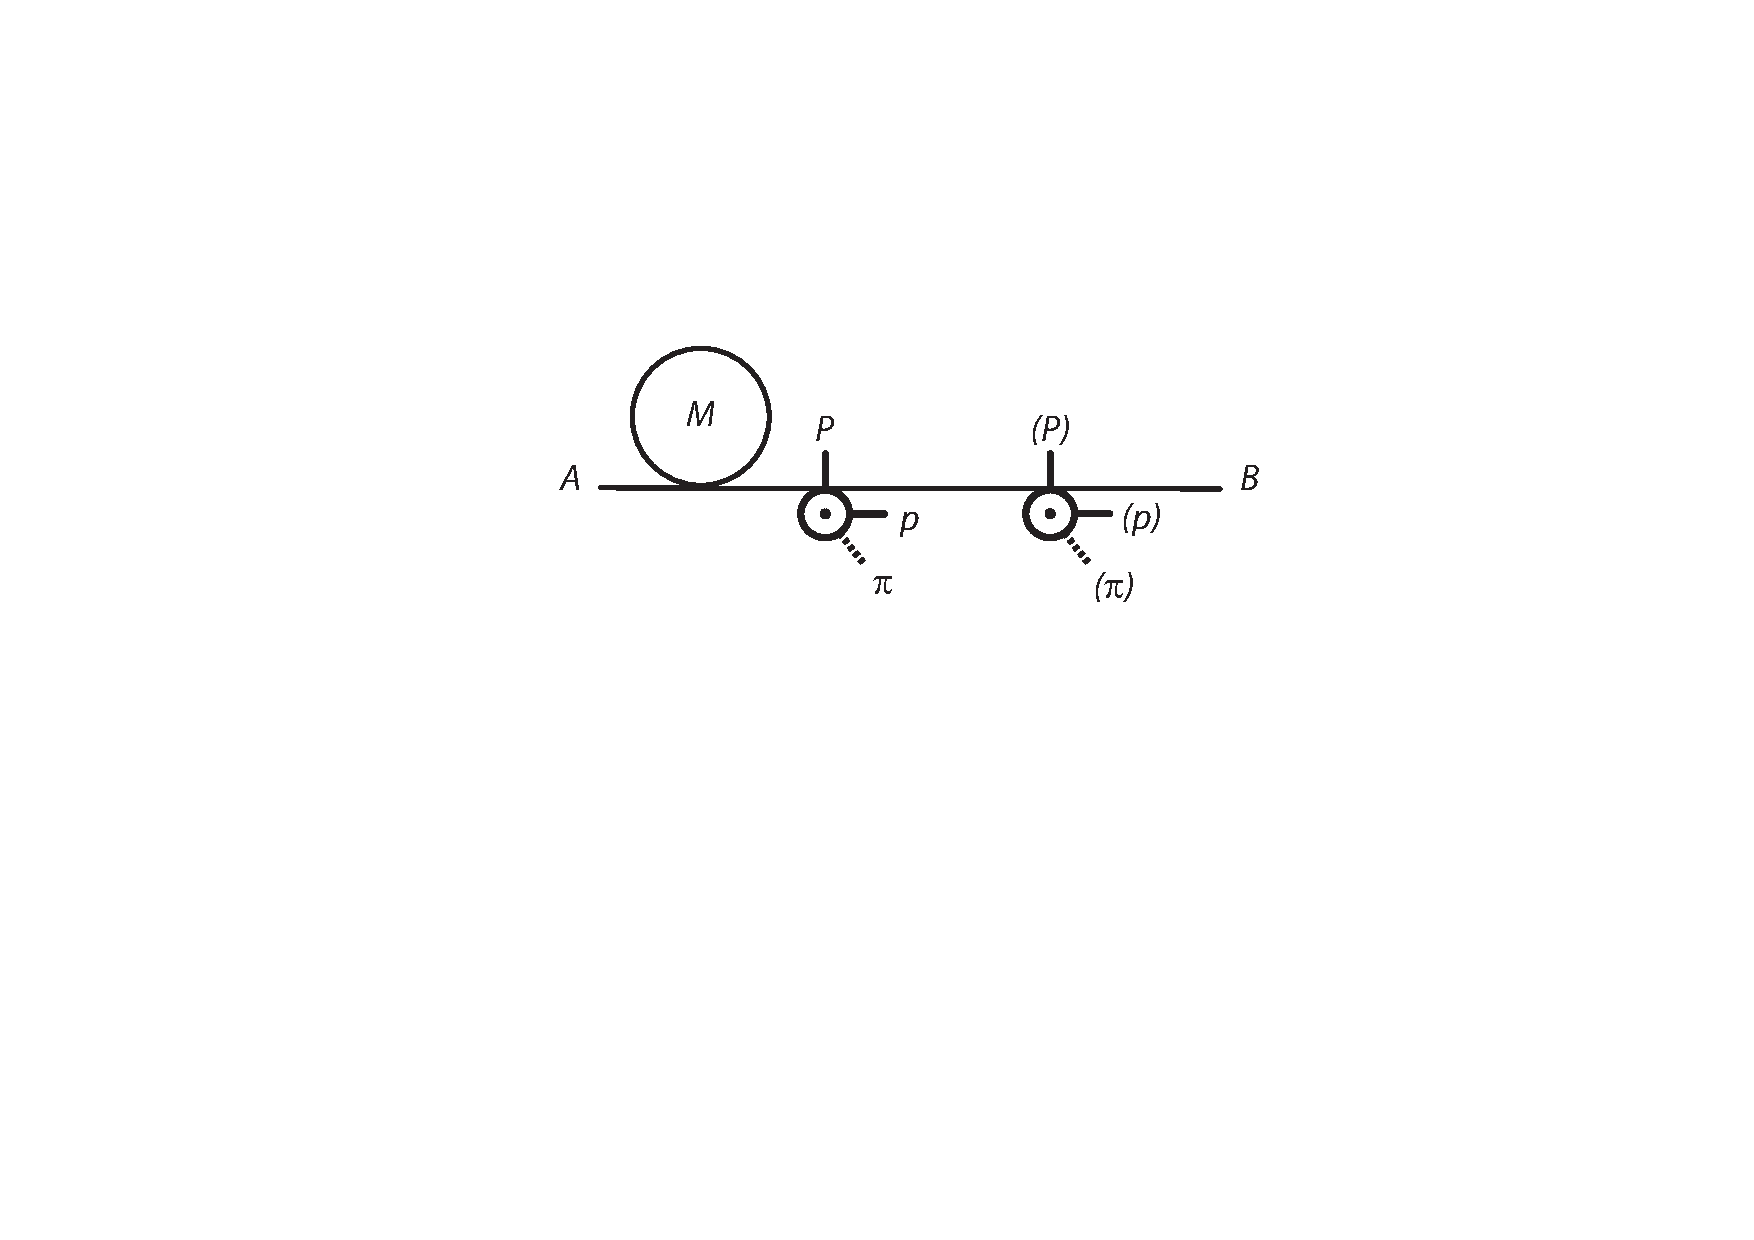
\includegraphics[trim = 0mm -3mm 0mm 0mm, clip, width=0.55\textwidth]{images/lh03705_127v-d1.pdf}
    \pend
    \pstart
    \noindent
\centering
   [\textit{Fig. 1}] %\caption{Bildbeschreibung} 
    %\end{wrapfigure}
\pend
\count\Bfootins=1500
\count\Cfootins=1500
\count\Afootins=1500